% ================================================================
%  CHƯƠNG 2 — CƠ SỞ LÝ THUYẾT
% ================================================================

% ----------------------------------------------------------------
\section{Tổng quan về bài toán và dữ liệu}
\label{sec:bg-data}

\subsection{Biểu diễn dữ liệu hình ảnh và không gian màu YCbCr}
\label{ssec:ycbcr}

Ảnh kỹ thuật số được biểu diễn dưới dạng ma trận số nguyên hai chiều (ảnh xám) hoặc ba chiều (ảnh màu). Mỗi phần tử của ma trận (gọi là điểm ảnh, pixel) lưu giá trị cường độ ánh sáng trong khoảng $[0, 255]$ với định dạng 8-bit, hoặc $[0, 1]$ sau khi chuẩn hóa. Trong bài toán tổng hợp ảnh, hầu hết các phương pháp xử lý ảnh xám (thang độ xám, một kênh) vì mỗi modality y tế về cơ bản là bản đồ cường độ đơn kênh.

Tuy nhiên, đối với ảnh PET và SPECT, thông tin chức năng thường được trực quan hóa bằng bản đồ màu giả (pseudo-color) nhằm giúp bác sĩ phân biệt các vùng hoạt động chuyển hóa. Trong trường hợp này, mô hình cần xử lý ảnh màu mà vẫn bảo toàn thông tin cường độ gốc. Đây là lý do không gian màu YCbCr được ứng dụng rộng rãi trong xử lý ảnh y tế tổng hợp.

\paragraph{Không gian màu YCbCr.}
YCbCr là không gian màu tách biệt thành phần độ chói (luminance) $Y$ và hai thành phần độ màu sắc (chrominance) $C_b$, $C_r$:
\begin{equation}
\begin{bmatrix} Y \\ C_b \\ C_r \end{bmatrix}
=
\begin{bmatrix} 0.299 & 0.587 & 0.114 \\ -0.169 & -0.331 & 0.500 \\ 0.500 & -0.419 & -0.081 \end{bmatrix}
\begin{bmatrix} R \\ G \\ B \end{bmatrix}
+
\begin{bmatrix} 0 \\ 128 \\ 128 \end{bmatrix}
\label{eq:ycbcr}
\end{equation}
trong đó $Y \in [16, 235]$ mang toàn bộ thông tin cấu trúc không gian (tương đương ảnh xám), còn $C_b$, $C_r \in [16, 240]$ chỉ mang thông tin màu sắc mà không ảnh hưởng đến độ sắc nét.

Khi tổng hợp ảnh PET--MRI hoặc SPECT--MRI với đầu vào màu, chiến lược phổ biến là:
\begin{enumerate}\itemsep2pt
    \item Chuyển ảnh màu (PET/SPECT) sang không gian YCbCr.
    \item Chỉ đưa kênh $Y$ (luminance) vào mô hình fusion cùng với ảnh MRI xám.
    \item Sau khi tổng hợp, gán kênh $Y$ tổng hợp vào cặp $(C_b, C_r)$ của ảnh gốc rồi chuyển ngược về RGB.
\end{enumerate}
Chiến lược này giữ nguyên màu sắc đặc trưng của PET/SPECT (màu nóng/lạnh biểu thị mức độ hoạt động) trong khi thông tin cấu trúc từ MRI được đưa vào qua kênh luminance. CDDFuse và hầu hết các phương pháp MIF hiện đại đều áp dụng chiến lược này cho ảnh màu. Hình~\ref{fig:ycbcr} minh họa quá trình chuyển đổi và tách kênh trên một ảnh PET thực tế từ tập Harvard.

\begin{figure}[H]
    \centering
    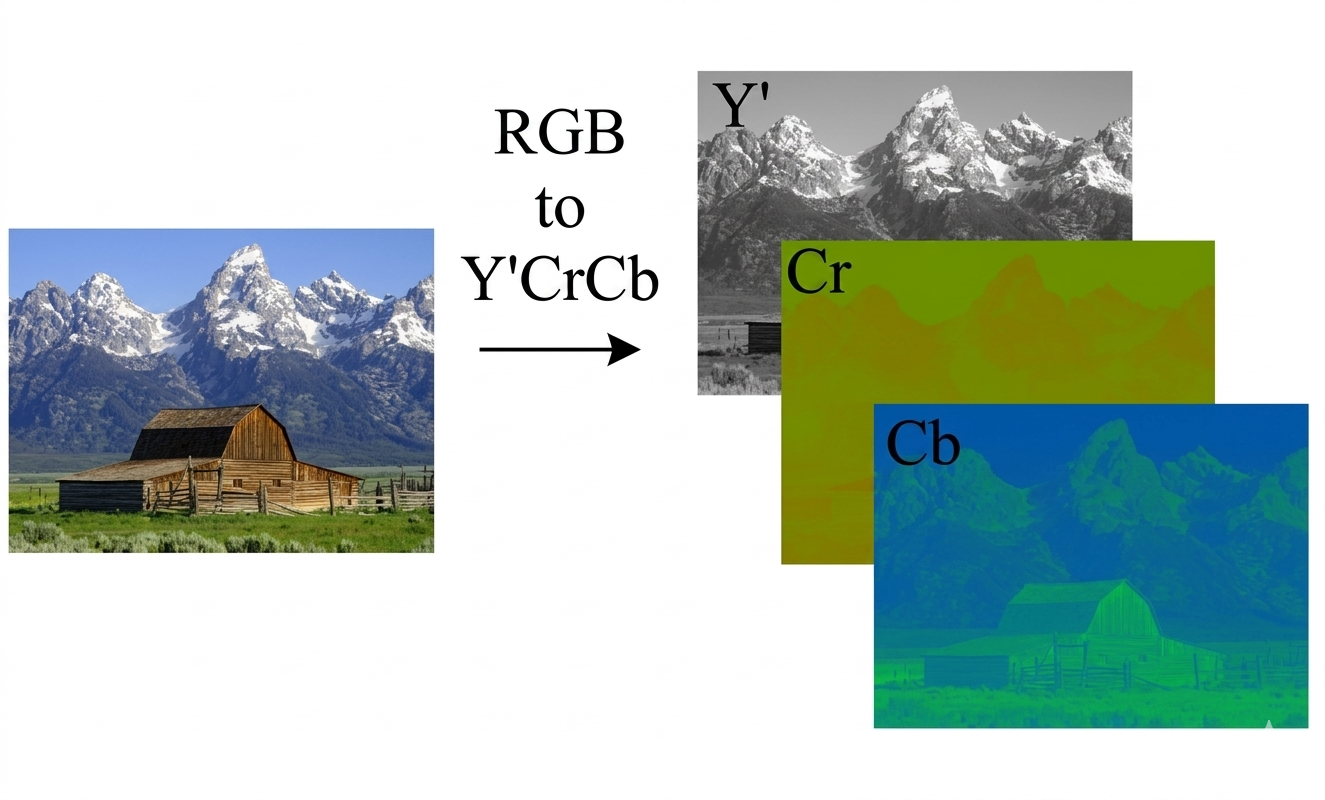
\includegraphics[width=0.7\textwidth]{figures/fig_ycbcr.png}
    \caption{Chuyển đổi RGB sang YCbCr và tách thành ba kênh Y (độ chói), Cb (sắc xanh) và Cr (sắc đỏ).}
    \label{fig:ycbcr}
\end{figure}

\paragraph{Chuẩn hóa và xử lý tiền kỳ.}
Trước khi đưa vào mạng, ảnh được chuẩn hóa về khoảng $[0, 1]$ bằng phép chia cho 255. Trong quá trình huấn luyện, ảnh được cắt thành các patch $128 \times 128$ để đảm bảo tính đồng nhất đầu vào và giảm yêu cầu bộ nhớ GPU. Tại thời điểm kiểm thử (inference), ảnh gốc kích thước đầy đủ được đưa vào trực tiếp: CDDFuse xử lý ảnh theo từng cặp độc lập, không yêu cầu padding hay resize.

% ----------------------------------------------------------------
\subsection{Các phương thức ảnh y tế}
\label{ssec:modalities}

Bốn phương thức ảnh y tế chính được sử dụng trong đồ án có đặc điểm vật lý và thông tin bổ sung cho nhau~\cite{liu2018survey}, được tóm tắt trong Bảng~\ref{tab:modalities}.

\begin{table}[H]
\centering
\small
\caption{So sánh bốn phương thức ảnh y tế sử dụng trong đồ án.}
\label{tab:modalities}
\setlength{\tabcolsep}{5pt}
\renewcommand{\arraystretch}{1.4}
\footnotesize
\begin{tabular}{|>{\centering\arraybackslash}m{0.12\textwidth}|>{\centering\arraybackslash}m{0.15\textwidth}|m{0.19\textwidth}|m{0.19\textwidth}|m{0.16\textwidth}|}
\hline
\textbf{Phương thức} & \textbf{Ảnh mẫu} & \centering\textbf{Nguyên lý} & \centering\textbf{Thông tin cung cấp} & \centering\arraybackslash\textbf{Hạn chế} \\
\hline
\textbf{CT}
(Chụp cắt lớp vi tính)
&
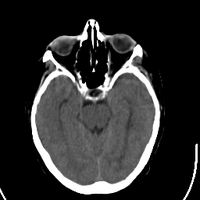
\includegraphics[width=0.14\textwidth]{figures/modality_samples/CT.png}
&
Đo mức hấp thụ tia X của các mô. Xương hấp thụ nhiều → pixel sáng; mô mềm và không khí → pixel tối.
&
Cấu trúc xương, mô đặc, canxi hóa rõ nét. Tốt cho chẩn đoán gãy xương, u xương.
&
Phân giải mô mềm thấp. Bệnh nhân tiếp xúc tia X. \\
\hline
\textbf{MRI}
(Chụp cộng hưởng từ)
&
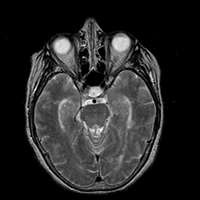
\includegraphics[width=0.14\textwidth]{figures/modality_samples/MRI.png}
&
Tín hiệu từ hạt nhân hydrogen trong nước và mỡ khi đặt trong từ trường mạnh.
&
Phân giải mô mềm vượt trội: não, tủy sống, cơ, dây chằng. Không dùng tia X.
&
Thời gian chụp lâu. Chống chỉ định với bệnh nhân có kim loại trong người. \\
\hline
\textbf{PET}
(Chụp cắt lớp phát xạ positron)
&
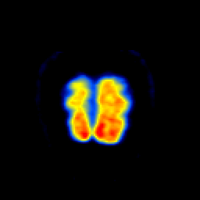
\includegraphics[width=0.14\textwidth]{figures/modality_samples/PET.png}
&
Đo hoạt động chuyển hóa qua chất đánh dấu phóng xạ (FDG, glucose). Vùng hoạt động mạnh → cường độ cao.
&
Thông tin chức năng--phân tử: phát hiện khối u, đánh giá thần kinh.
&
Độ phân giải không gian thấp (${\sim}4$--$6$ mm). Chi phí cao. \\
\hline
\textbf{SPECT}
(Chụp cắt lớp đơn photon)
&
\vspace{4pt}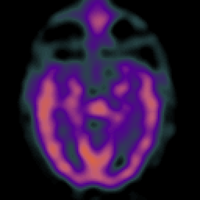
\includegraphics[width=0.14\textwidth]{figures/modality_samples/SPECT.png}\vspace{2pt}
&
Tương tự PET nhưng dùng chất đánh dấu phát tia gamma một photon.
&
Lưu lượng máu não và tim. Chi phí thấp hơn PET, thiết bị phổ biến hơn.
&
Độ phân giải kém hơn PET (${\sim}8$--$10$ mm). Thời gian chụp dài. \\
\hline
\end{tabular}
\end{table}

Sự bổ trợ thông tin giữa các modality tạo ra nhu cầu tự nhiên cho bài toán tổng hợp: CT--MRI kết hợp cấu trúc xương (CT) với cấu trúc mô mềm (MRI); PET--MRI và SPECT--MRI kết hợp thông tin chức năng (PET/SPECT) với thông tin giải phẫu (MRI).

% ----------------------------------------------------------------
% ================================================================
\section{Nền tảng kiến trúc học sâu}
\label{sec:bg-dl}

\subsection{Mạng tích chập và cơ chế Attention}
\label{ssec:cnn-attention}

\paragraph{Mạng tích chập (CNN).}
Mạng nơ-ron tích chập là nền tảng của xử lý ảnh hiện đại~\cite{lecun1998gradient}. Phép tích chập 2D áp dụng bộ lọc (kernel) $k \in \mathbb{R}^{K \times K}$ trượt qua ảnh đầu vào để trích xuất đặc trưng cục bộ:
\begin{equation}
(I * k)[i, j] = \sum_{m=0}^{K-1} \sum_{n=0}^{K-1} I[i+m, j+n] \cdot k[m, n]
\end{equation}
Bằng cách xếp chồng nhiều lớp tích chập xen kẽ với hàm kích hoạt phi tuyến (ReLU, LeakyReLU), mạng CNN học được các đặc trưng từ đơn giản (biên, góc) đến phức tạp (cấu trúc giải phẫu). Hình~\ref{fig:conv-demo} minh họa cụ thể một phép tích chập với kernel Laplacian phát hiện biên.

\begin{figure}[H]
    \centering
    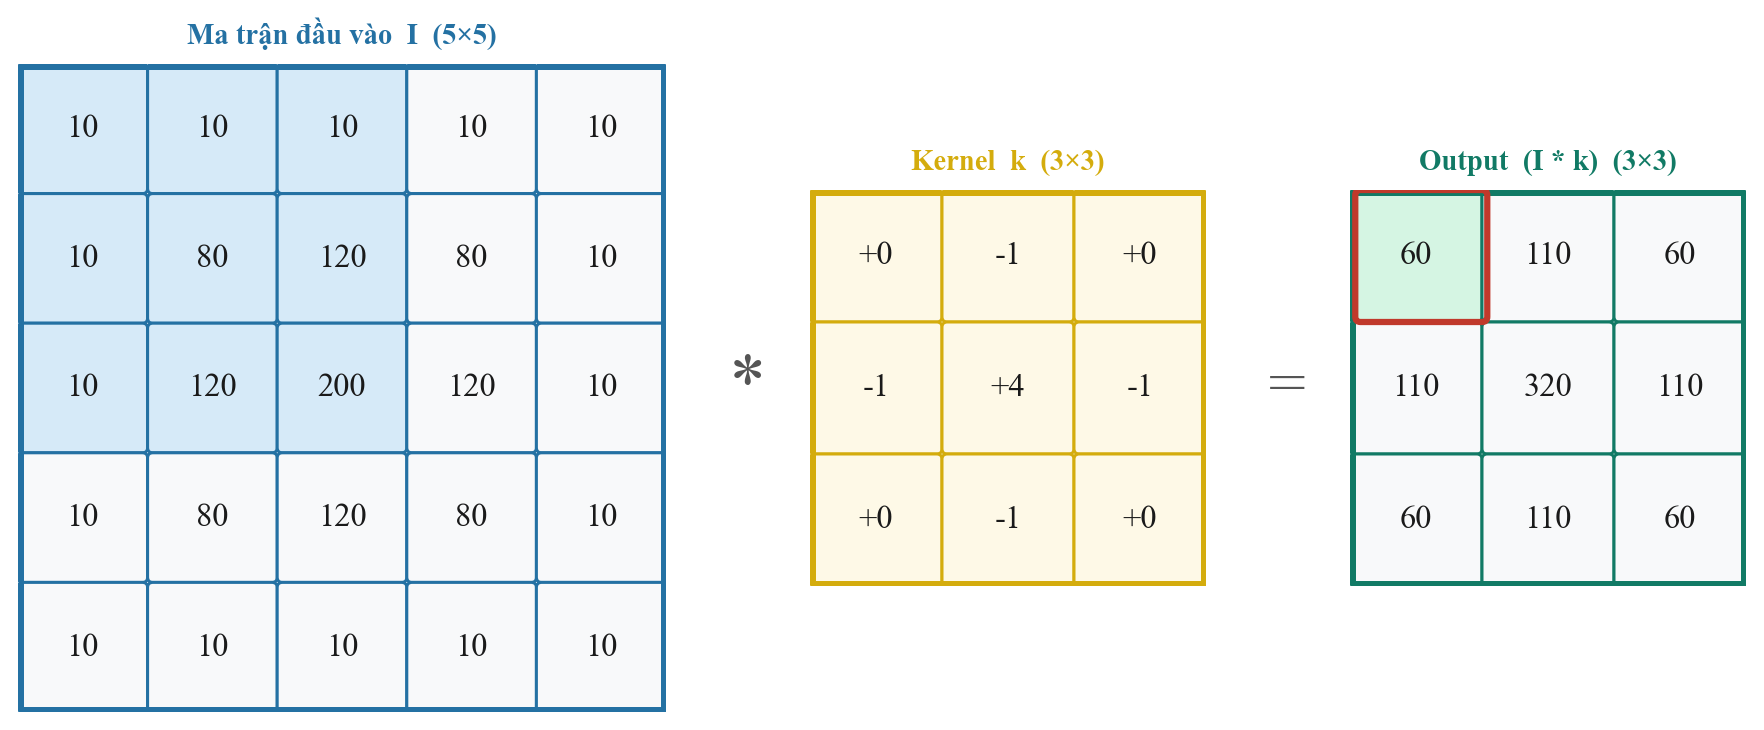
\includegraphics[width=0.65\textwidth]{figures/fig_conv_demo.png}
    \caption{Minh họa phép tích chập 2D: kernel Laplacian $3\times3$ trượt qua ảnh $5\times5$, sinh feature map $3\times3$.}
    \label{fig:conv-demo}
\end{figure} Tuy nhiên, CNN có vùng tiếp nhận (receptive field) hữu hạn, khó nắm bắt phụ thuộc tầm xa giữa các vùng xa nhau trong ảnh.

\paragraph{Cơ chế Attention.}
Để khắc phục giới hạn tầm xa của CNN, cơ chế attention cho phép mô hình tự hỏi: ``Với vị trí này trong ảnh, tôi nên nhìn vào đâu để lấy thông tin?'' Ý tưởng tương tự như tra cứu từ điển: có một câu hỏi (query), một tập khóa (key) gắn với từng vị trí, và giá trị (value) tương ứng với mỗi khóa.

Cụ thể, đặc trưng đầu vào được chiếu tuyến tính thành ba ma trận:
\begin{itemize}\itemsep1pt
    \item $Q$ (Query): ``tôi đang tìm kiếm thông tin gì?''
    \item $K$ (Key): ``mỗi vị trí trong ảnh chứa thông tin gì?''
    \item $V$ (Value): thông tin thực sự được lấy ra từ mỗi vị trí.
\end{itemize}

Mức độ liên quan giữa một query và tất cả các key được tính bằng tích vô hướng $QK^\top$, sau đó chia cho $\sqrt{d_k}$ để tránh giá trị quá lớn làm gradient bão hòa. Hàm softmax chuyển các điểm số này thành trọng số chú ý (attention weights) tổng bằng 1, thể hiện ``tôi quan tâm đến vị trí kia bao nhiêu phần trăm''. Cuối cùng, các giá trị $V$ được tổng hợp có trọng số~\cite{vaswani2017attention}:
\begin{equation}
\mathrm{Attention}(Q, K, V) = \mathrm{softmax}\!\left(\frac{QK^\top}{\sqrt{d_k}}\right) V
\end{equation}

Multi-head Attention chạy $h$ phép attention song song với không gian chiếu khác nhau, sau đó nối kết quả lại. Mỗi head học một kiểu phụ thuộc khác nhau: một head có thể học quan hệ cạnh-cạnh, head khác học quan hệ vùng xa, tổng hợp lại cho mô hình cái nhìn toàn diện hơn CNN thuần túy. Hình~\ref{fig:attention} minh họa luồng tính toán đầy đủ.

\begin{figure}[H]
    \centering
    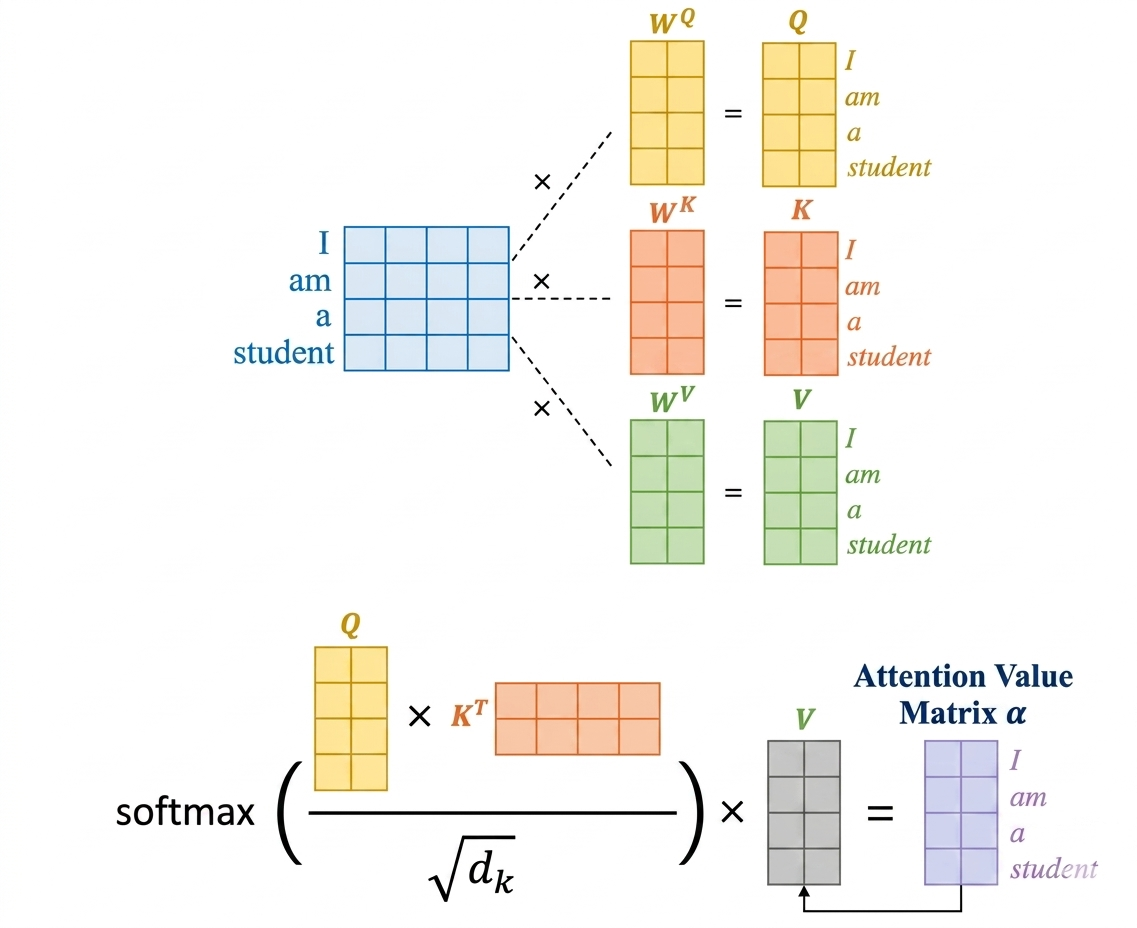
\includegraphics[width=0.8\textwidth]{figures/scale_dot_product_attention.png}
    \caption[Sơ đồ Scaled Dot-Product Attention]{Sơ đồ Scaled Dot-Product Attention: $Q$, $K$, $V$ qua các bước nhân ma trận, chia tỉ lệ và softmax để tạo ra đặc trưng đầu ra. (Nguồn: \cite{vaswani2017attention})}
    \label{fig:attention}
\end{figure}

% ----------------------------------------------------------------
\subsection{Transformer và Restormer Encoder}
\label{ssec:transformer}

\paragraph{Vision Transformer (ViT).}
Transformer ban đầu được thiết kế cho xử lý ngôn ngữ tự nhiên, nhưng đã được chuyển đổi thành công sang xử lý ảnh bởi Dosovitskiy et al.~\cite{dosovitskiy2020vit}. Ý tưởng cốt lõi là coi mỗi patch nhỏ của ảnh như một token từ trong câu, từ đó áp dụng Transformer encoder không thay đổi.

Bước 1: Patch Embedding.
Ảnh đầu vào $\mathbf{x} \in \mathbb{R}^{H \times W \times C}$ được chia thành $N$ patch không chồng lấp kích thước $P \times P$, mỗi patch được phẳng hóa và chiếu tuyến tính thành vector $d$-chiều:
\begin{equation}
\mathbf{z}_i^{(0)} = \mathbf{E} \cdot \mathrm{flatten}(\mathbf{x}_i) + \mathbf{p}_i, \quad i = 1, \ldots, N
\label{eq:patch-embed}
\end{equation}
trong đó $\mathbf{E} \in \mathbb{R}^{d \times (P^2 C)}$ là ma trận chiếu học được, $N = HW/P^2$ là số patch, và $\mathbf{p}_i \in \mathbb{R}^d$ là positional embedding (vector học được mã hóa vị trí không gian của patch thứ $i$, vì self-attention không có khái niệm thứ tự vốn có).

Bước 2: Transformer Encoder Block.
Chuỗi $N$ token đi qua $L$ block xếp nối tiếp, mỗi block gồm hai thành phần chính với kết nối dư (residual):
\begin{align}
\mathbf{z}'^{(\ell)} &= \mathrm{MSA}\!\left(\mathrm{LN}(\mathbf{z}^{(\ell-1)})\right) + \mathbf{z}^{(\ell-1)} \label{eq:vit-msa} \\
\mathbf{z}^{(\ell)}  &= \mathrm{MLP}\!\left(\mathrm{LN}(\mathbf{z}'^{(\ell)})\right) + \mathbf{z}'^{(\ell)} \label{eq:vit-mlp}
\end{align}
trong đó:
\begin{itemize}\itemsep1pt
    \item $\mathrm{LN}$: Layer Normalization, chuẩn hóa từng token theo chiều đặc trưng, ổn định huấn luyện.
    \item $\mathrm{MSA}$: Multi-head Self-Attention, mỗi token đồng thời làm query và key/value cho tất cả token còn lại, cho phép học phụ thuộc tầm xa toàn cục $O(N^2)$.
    \item $\mathrm{MLP}$: hai lớp fully-connected với hàm kích hoạt GELU, chiều ẩn thường $= 4d$.
    \item Kết nối dư (residual $+$): giữ nguyên thông tin từ lớp trước, tránh mất mát gradient ở mạng sâu.
\end{itemize}

Độ phức tạp tính toán.
Vì MSA tính tương tác giữa mọi cặp token, chi phí tăng bậc hai theo số token:
\begin{equation}
\mathcal{C}_{\mathrm{SA}} = O(N^2 d) = O\!\left(\frac{(HW)^2}{P^4}\,d\right)
\label{eq:vit-complexity}
\end{equation}
Kích thước patch $P$ vì vậy là tham số then chốt: tăng $P$ lên 2 lần thì chi phí giảm 16 lần. Hình~\ref{fig:vit-complexity} minh họa cụ thể với ảnh $256\times256$, $d=768$:

\begin{figure}[H]
    \centering
    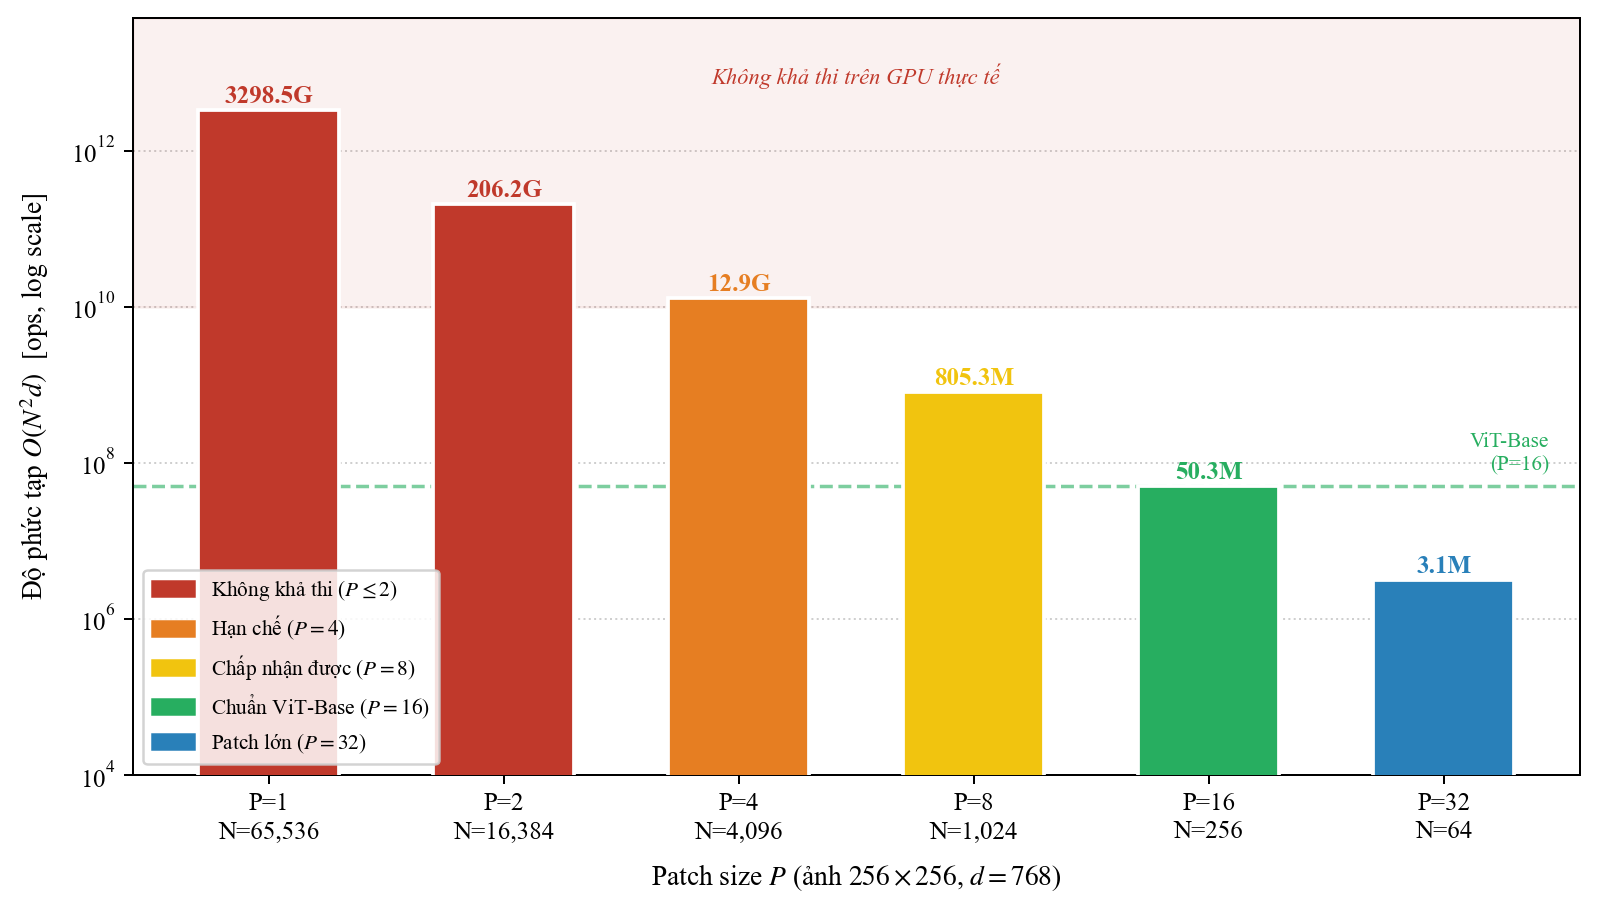
\includegraphics[width=0.82\textwidth]{figures/fig_vit_complexity.png}
    \caption{Độ phức tạp $O(N^2d)$ theo kích thước patch $P$ (thang log). $P=16$ là điểm cân bằng giữa hiệu quả tính toán và khả năng mô hình hóa chi tiết cục bộ.}
    \label{fig:vit-complexity}
\end{figure}

Đây là lý do Restormer (xem bên dưới) chuyển attention từ chiều không gian sang chiều kênh, phá vỡ nút thắt cổ chai $O((HW)^2)$ khi xử lý ảnh y tế độ phân giải cao.

\paragraph{Restormer.}
Restormer~\cite{zamir2022restormer} (Restoration Transformer) là kiến trúc Transformer được thiết kế đặc biệt để khôi phục ảnh độ phân giải cao, giải quyết nút thắt cổ chai tính toán của ViT bằng hai cải tiến cốt lõi.

Multi-Dconv Head Transposed Attention (MDTA).
Thay vì tính attention trên chiều không gian (mỗi pixel là một token), MDTA tính attention trên chiều kênh. Cụ thể, với đặc trưng đầu vào $\mathbf{X} \in \mathbb{R}^{C \times H \times W}$:
\begin{enumerate}\itemsep1pt
    \item Sinh $Q, K, V$ bằng tích chập sâu (depthwise conv $3\!\times\!3$) thay vì projection tuyến tính, giúp gộp thêm thông tin không gian cục bộ vào mỗi token kênh.
    \item Reshape: $Q, K, V \in \mathbb{R}^{\hat{C} \times HW}$ (mỗi kênh là một vector $HW$-chiều).
    \item Tính attention map trên ma trận $\hat{C} \times \hat{C}$ thay vì $HW \times HW$:
\end{enumerate}
\begin{equation}
\mathrm{MDTA}(\mathbf{X}) = \mathrm{Attention}(Q K^\top / \alpha)\, V, \quad
\text{attention map } \in \mathbb{R}^{\hat{C} \times \hat{C}}
\label{eq:mdta}
\end{equation}
trong đó $\alpha$ là tham số scale học được. So sánh độ phức tạp:
\[
\underbrace{O\!\left((HW)^2 C\right)}_{\text{Spatial attention (ViT)}}
\;\longrightarrow\;
\underbrace{O\!\left(C^2 HW\right)}_{\text{Channel attention (MDTA)}}
\]
\begin{tcolorbox}[
    enhanced, arc=5pt, boxrule=1.2pt,
    colback=blue!4!white, colframe=blue!35!black,
    left=10pt, right=10pt, top=6pt, bottom=6pt
]
\centering
\small
\begin{tabular}{lcc}
    & \textbf{Spatial Attention (ViT)} & \textbf{MDTA (Restormer)} \\[3pt]
    \hline\\[-6pt]
    Attention map & $HW \times HW = 65536^2$ & $C \times C = 64^2$ \\[2pt]
    Độ phức tạp   & $O\!\left((HW)^2 C\right)$ & $O\!\left(C^2\, HW\right)$ \\[2pt]
    Số ops (ảnh $256^2$, $C\!=\!64$) & $\sim 2.7\times10^{11}$ & $\sim 2.7\times10^{8}$ \\[4pt]
    \hline\\[-6pt]
    \multicolumn{3}{c}{\normalsize MDTA nhanh hơn $\approx$1000 lần so với Spatial Attention}
\end{tabular}
\end{tcolorbox}

Gated-Dconv Feed-Forward Network (GDFN).
Thay thế MLP thông thường trong Transformer bằng mạng có cơ chế gating:
\begin{equation}
\mathrm{GDFN}(\mathbf{X}) = \phi\!\left(\mathrm{DConv}(W_1 \mathbf{X})\right) \odot \mathrm{DConv}(W_2 \mathbf{X})
\label{eq:gdfn}
\end{equation}
trong đó $\phi$ là GELU, $\odot$ là nhân theo phần tử (element-wise), và $W_1, W_2$ là tích chập $1\!\times\!1$. Cơ chế gating cho phép mạng kiểm soát chủ động luồng đặc trưng nào được truyền tiếp: nhánh trái học ``nên giữ thông tin gì'', nhánh phải học ``thông tin nào cần lọc bỏ''.

Cấu trúc một Restormer Block.
Mỗi block gồm hai bước với kết nối dư, tương tự ViT nhưng thay MSA bằng MDTA và MLP bằng GDFN:
\begin{align}
\mathbf{X}' &= \mathrm{MDTA}\!\left(\mathrm{LN}(\mathbf{X})\right) + \mathbf{X} \\
\mathbf{X}'' &= \mathrm{GDFN}\!\left(\mathrm{LN}(\mathbf{X}')\right) + \mathbf{X}'
\end{align}

CDDFuse sử dụng Restormer block làm xương sống cho cả Encoder và Decoder, cho phép mô hình học phụ thuộc tầm xa giữa các kênh đặc trưng ảnh y tế mà vẫn đảm bảo hiệu quả tính toán.

% ----------------------------------------------------------------
\subsection{Mạng nơ-ron khả nghịch (INN)}
\label{ssec:inn}

\paragraph{Vấn đề mất thông tin trong CNN thông thường.}
Mạng CNN thông thường thực hiện ánh xạ một chiều $f: \mathbf{x} \to \mathbf{y}$. Một khi đặc trưng $\mathbf{y}$ đã được tính, không thể khôi phục lại $\mathbf{x}$ gốc, vì thông tin đã bị nén và mất đi không thể đảo ngược. Với ảnh y tế, điều này có nghĩa là các chi tiết biên mỏng (ví dụ ranh giới khối u trong MRI) có thể bị lọc mất qua các lớp convolution.

\paragraph{Ý tưởng cốt lõi của INN.}
Mạng nơ-ron khả nghịch (\emph{Invertible Neural Network}, INN) xây dựng ánh xạ $f$ sao cho luôn tồn tại $f^{-1}$ tính được hiệu quả:
\[
\mathbf{x} \;\xrightarrow{f}\; \mathbf{y} \;\xrightarrow{f^{-1}}\; \mathbf{x}
\]
Không có thông tin nào bị mất: toàn bộ nội dung của $\mathbf{x}$ được mã hóa trong $\mathbf{y}$ và có thể phục hồi hoàn toàn. CDDFuse sử dụng INN cho nhánh Detail CNN Encoder để đảm bảo thông tin modality-specific (tần số cao) không bị mất khi mã hóa.

\paragraph{Affine Coupling Layer (RealNVP).}
Câu hỏi thực tế là: làm thế nào để xây dựng được $f$ khả nghịch mà không cần $f$ phải có dạng đặc biệt? RealNVP~\cite{dinh2017density} trả lời bằng thủ thuật chia đôi và coupling (\emph{affine coupling layer}):

Bước 1: Chia đôi đầu vào.
Đặc trưng $\mathbf{x} \in \mathbb{R}^{2C \times H \times W}$ được chia thành hai nửa $(\mathbf{x}_1, \mathbf{x}_2) \in \mathbb{R}^{C \times H \times W}$ (chia theo chiều kênh).

Bước 2: Biến đổi có điều kiện (chiều thuận).
Nửa $\mathbf{x}_1$ được biến đổi có điều kiện trên $\mathbf{x}_2$, và ngược lại:
\begin{align}
\mathbf{y}_1 &= \mathbf{x}_1 \odot \exp\!\bigl(s_1(\mathbf{x}_2)\bigr) + t_1(\mathbf{x}_2) \label{eq:inn-fwd1} \\
\mathbf{y}_2 &= \mathbf{x}_2 \odot \exp\!\bigl(s_2(\mathbf{y}_1)\bigr) + t_2(\mathbf{y}_1) \label{eq:inn-fwd2}
\end{align}
trong đó $s_i(\cdot)$ (scale) và $t_i(\cdot)$ (translation) là các mạng CNN con tùy ý, không cần phải khả nghịch. Phép nhân $\odot \exp(s)$ là phép nhân theo phần tử, có tác dụng co giãn từng kênh đặc trưng.

Bước 3: Nghịch đảo (chiều ngược).
Đây là phần then chốt: vì $\mathbf{y}_1$ đã biết, ta tính ngược từ dưới lên:
\begin{align}
\mathbf{x}_2 &= \bigl(\mathbf{y}_2 - t_2(\mathbf{y}_1)\bigr) \odot \exp\!\bigl(-s_2(\mathbf{y}_1)\bigr) \label{eq:inn-inv1} \\
\mathbf{x}_1 &= \bigl(\mathbf{y}_1 - t_1(\mathbf{x}_2)\bigr) \odot \exp\!\bigl(-s_1(\mathbf{x}_2)\bigr) \label{eq:inn-inv2}
\end{align}

\begin{figure}[H]
    \centering
    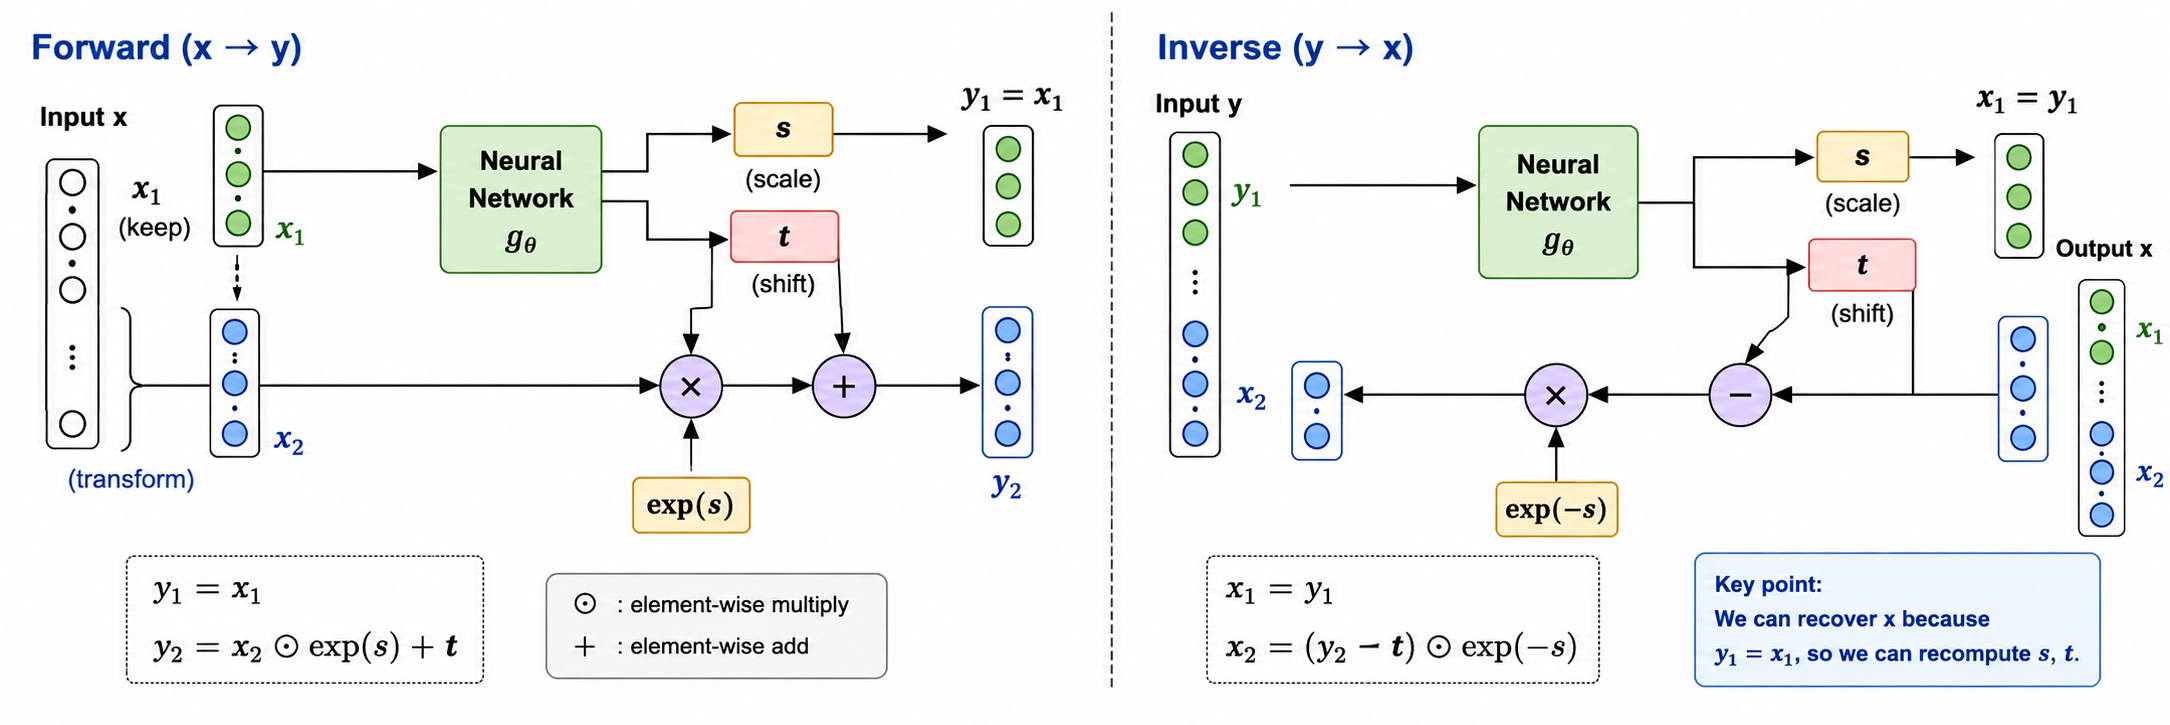
\includegraphics[width=0.975\textwidth]{figures/inn_block.png}
    \caption[Cấu trúc một khối INN (Affine Coupling Layer)]{Cấu trúc một khối INN (Affine Coupling Layer): chiều thuận (trái sang phải) và chiều nghịch (phải sang trái) đều tính được hiệu quả. (Nguồn: \cite{dinh2017density})}
    \label{fig:inn-block}
\end{figure}

\begin{tcolorbox}[
    enhanced, arc=5pt, boxrule=1pt,
    colback=green!4!white, colframe=green!40!black,
    left=9pt, right=9pt, top=5pt, bottom=5pt
]
Tại sao khả nghịch? Dù $s_i, t_i$ là mạng CNN bất kỳ, phép biến đổi toàn khối vẫn khả nghịch vì:
\begin{itemize}\itemsep1pt
    \item Phương trình~\eqref{eq:inn-fwd1} biến đổi $\mathbf{x}_1$ nhưng giữ nguyên $\mathbf{x}_2$ $\Rightarrow$ $\mathbf{x}_2$ vẫn đọc được từ $\mathbf{y}_2$ (bước đầu khi đảo ngược).
    \item Khi đã có $\mathbf{x}_2$, toàn bộ $s_1(\mathbf{x}_2)$ và $t_1(\mathbf{x}_2)$ đều tính được $\Rightarrow$ khôi phục $\mathbf{x}_1$ từ $\mathbf{y}_1$ theo công thức đại số đơn giản.
    \item Tính khả nghịch đến từ cấu trúc coupling, không phải từ $s_i, t_i$, do đó có thể dùng bất kỳ mạng nào cho $s_i, t_i$ mà không lo mất invertibility.
\end{itemize}
\end{tcolorbox}

\paragraph{Ứng dụng trong CDDFuse.}
Nhánh Detail CNN Encoder (DCE) gồm 3 khối coupling xếp nối tiếp. Mỗi ảnh đầu vào $I \in \mathbb{R}^{1 \times H \times W}$ được mở rộng lên 64 kênh qua tích chập rồi đi qua 3 lớp INN liên tiếp để thu đặc trưng detail $f^D \in \mathbb{R}^{64 \times H \times W}$. Tính khả nghịch đảm bảo mọi chi tiết tần số cao (biên mỏng, texture) đều được giữ nguyên trong $f^D$, điều mà CNN thông thường không đảm bảo được.

% ================================================================
\section{Mô hình CDDFuse}
\label{sec:cddfuse}

CDDFuse~\cite{zhao2023cddfuse} (CVPR 2023) là phương pháp tổng hợp ảnh đa phương thức dựa trên ý tưởng phân rã đặc trưng theo tương quan (\emph{Correlation-Driven Feature Decomposition}). Thay vì coi toàn bộ đặc trưng ảnh như một khối đồng nhất, CDDFuse phân rã chúng thành hai thành phần có bản chất khác nhau: Base (thông tin chung, tần số thấp) và Detail (thông tin đặc trưng từng modality, tần số cao), rồi thực hiện fusion riêng cho từng thành phần.

% ----------------------------------------------------------------
\subsection{Kiến trúc tổng quan}
\label{ssec:cddfuse-arch}

Mô hình gồm ba thành phần chính theo sơ đồ Encoder $\to$ Fuse $\to$ Decoder như minh họa trong Hình~\ref{fig:cddfuse-arch}.

\begin{figure}[H]
    \centering
    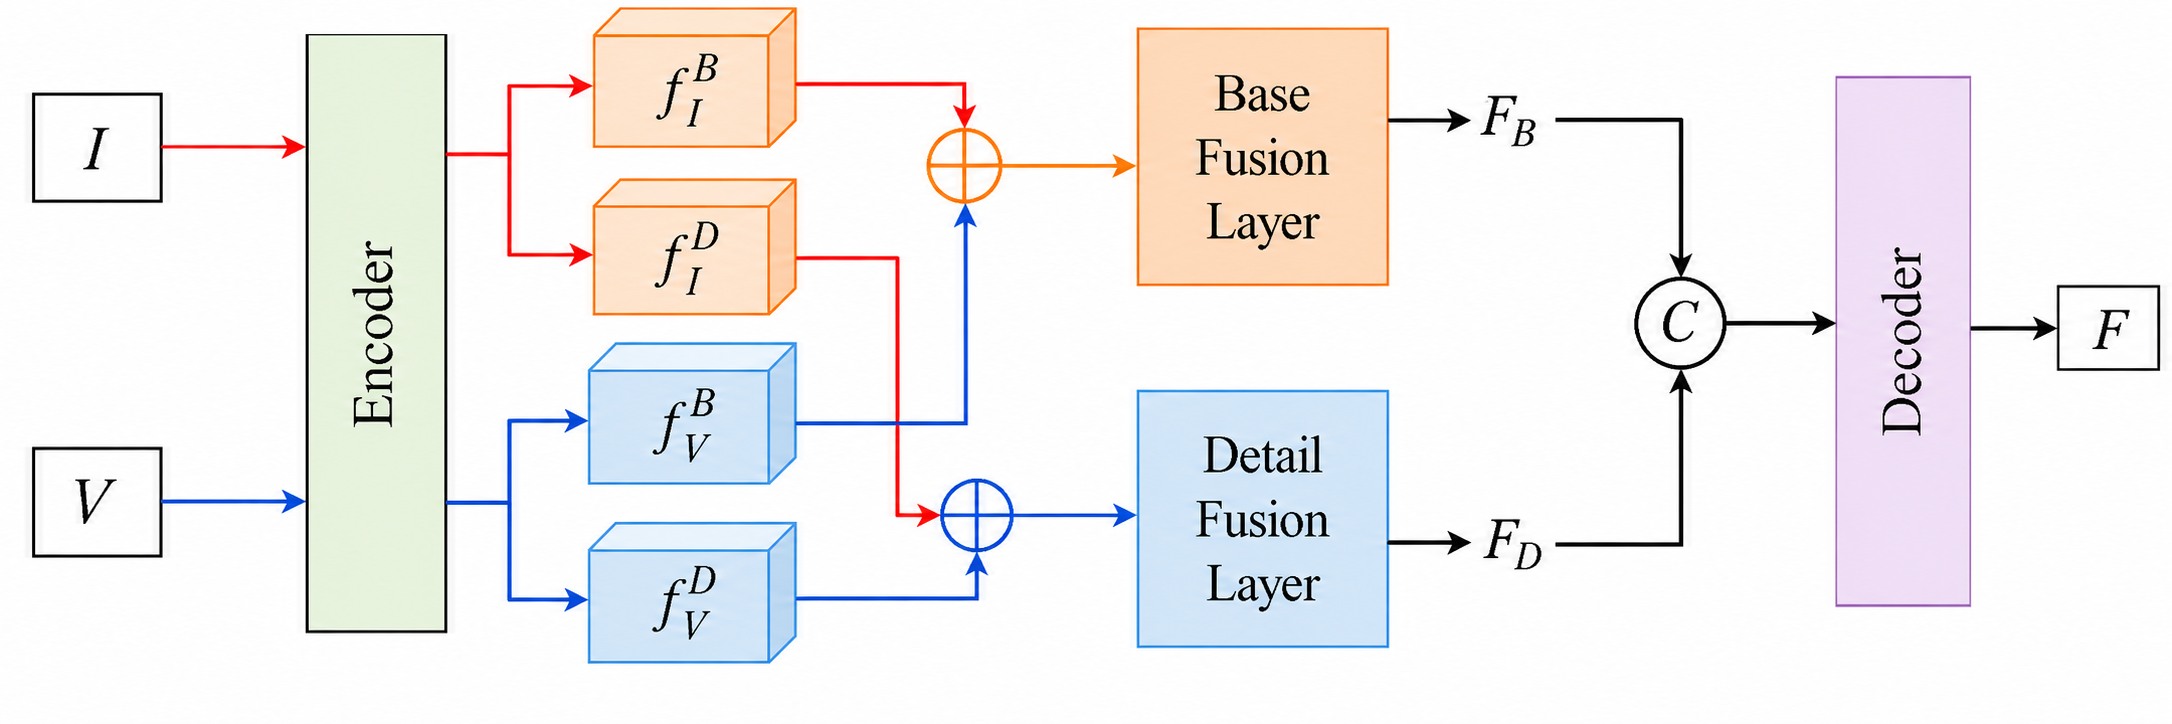
\includegraphics[width=\textwidth]{figures/cddfuse_pipeline.png}
    \caption[Kiến trúc tổng quan CDDFuse]{Kiến trúc tổng quan CDDFuse: hai ảnh đầu vào đi qua Encoder dùng chung trọng số, phân rã thành đặc trưng Base ($f^B$) và Detail ($f^D$), được tổng hợp riêng qua Fusion Layer, rồi giải mã thành ảnh đầu ra $I_F$. (Nguồn: \cite{zhao2023cddfuse})}
    \label{fig:cddfuse-arch}
\end{figure}

\paragraph{1. Restormer Encoder.}
Encoder dùng trọng số chung (shared weights) cho cả hai ảnh đầu vào $I_V$ và $I_I$, sinh ra hai cặp đặc trưng $(f_V^B, f_V^D)$ và $(f_I^B, f_I^D)$. Encoder gồm bốn bước:
\begin{itemize}\itemsep1pt
    \item Overlap Patch Embedding: tích chập $3\!\times\!3$ chuyển ảnh 1 kênh thành đặc trưng 64 kênh, giữ nguyên kích thước $H \times W$.
    \item Shallow Feature Extraction (SFE): 4 Restormer block xếp nối tiếp, học đặc trưng tầm xa qua MDTA.
    \item Base Transformer Encoder (BTE): một Restormer block với spatial multi-head attention, sinh đặc trưng $f^B \in \mathbb{R}^{64 \times H \times W}$.
    \item Detail CNN Encoder (DCE): 3 khối INN (RealNVP), sinh đặc trưng $f^D \in \mathbb{R}^{64 \times H \times W}$.
\end{itemize}

\begin{figure}[H]
    \centering
    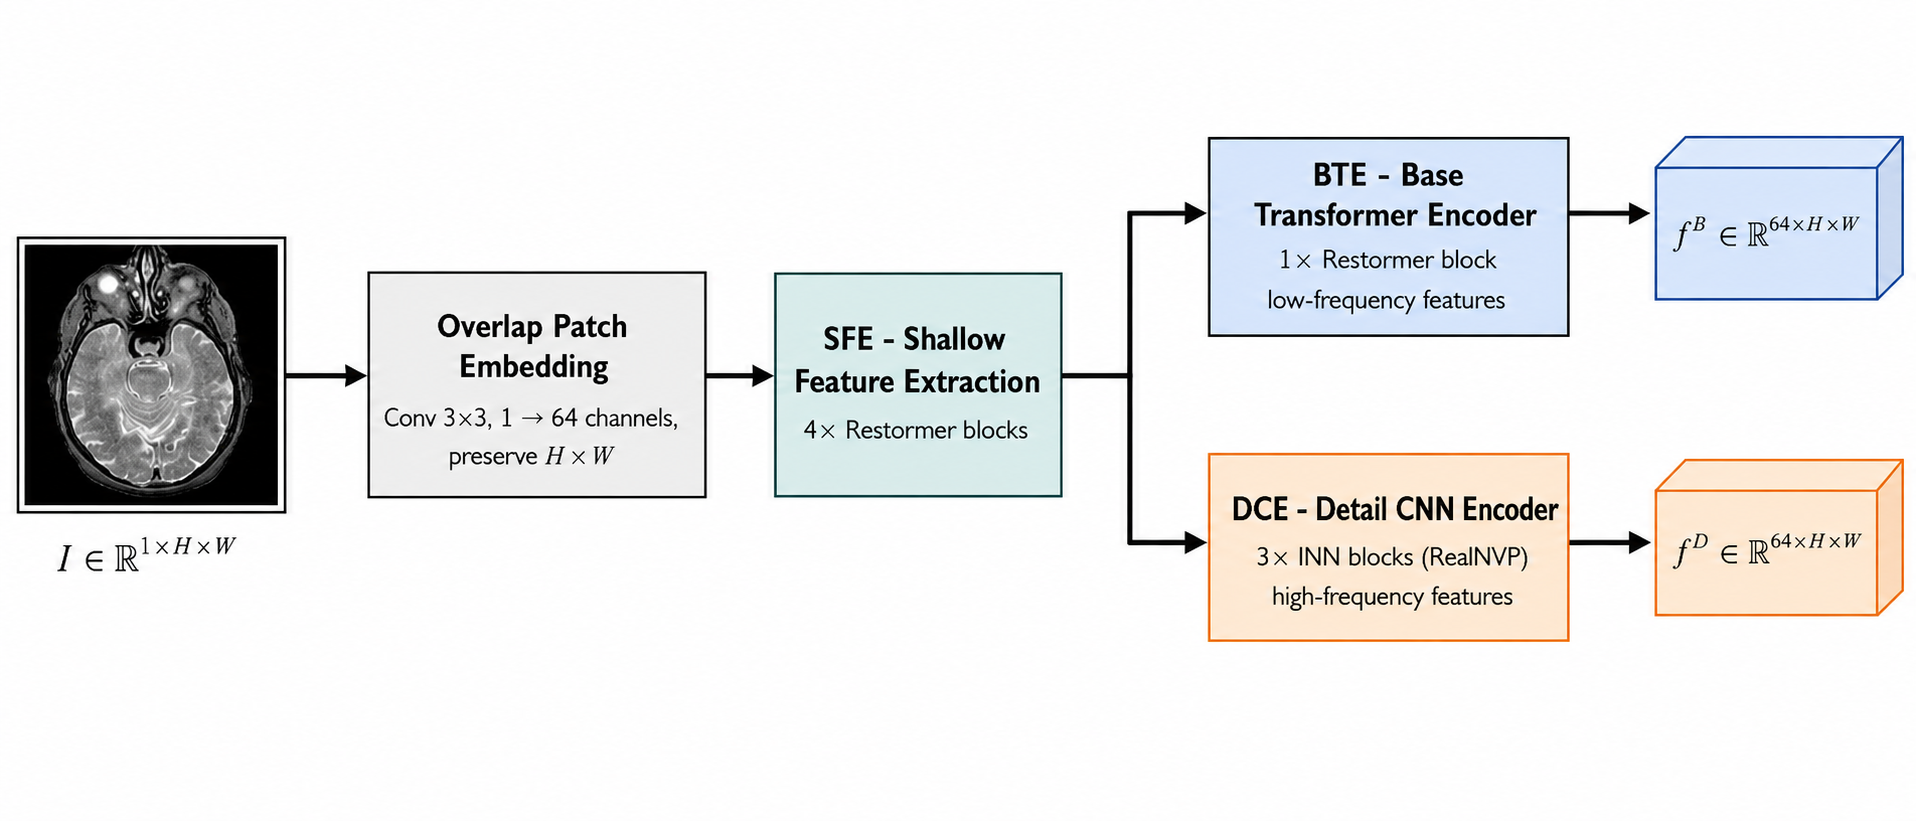
\includegraphics[width=\textwidth]{figures/encoder.png}
    \caption[Chi tiết kiến trúc Encoder CDDFuse]{Chi tiết kiến trúc Encoder CDDFuse: từ ảnh đầu vào qua Patch Embedding, SFE, rồi tách thành nhánh Base (BTE) và nhánh Detail (DCE). (Nguồn: \cite{zhao2023cddfuse})}
    \label{fig:cddfuse-encoder}
\end{figure}

\paragraph{2. Fusion Layer.}
Đặc trưng của hai modality được hợp nhất riêng cho từng nhánh:
\begin{align}
f_F^B &= \mathrm{BaseFuseLayer}(f_I^B + f_V^B) \label{eq:fuse-base} \\
f_F^D &= \mathrm{DetailFuseLayer}(f_I^D + f_V^D) \label{eq:fuse-detail}
\end{align}
Phép cộng $f_I + f_V$ trước khi qua layer là quy tắc tổng hợp đối xứng mặc định của CDDFuse, và đây chính là thành phần mà đồ án này cải tiến.

\begin{figure}[H]
    \centering
    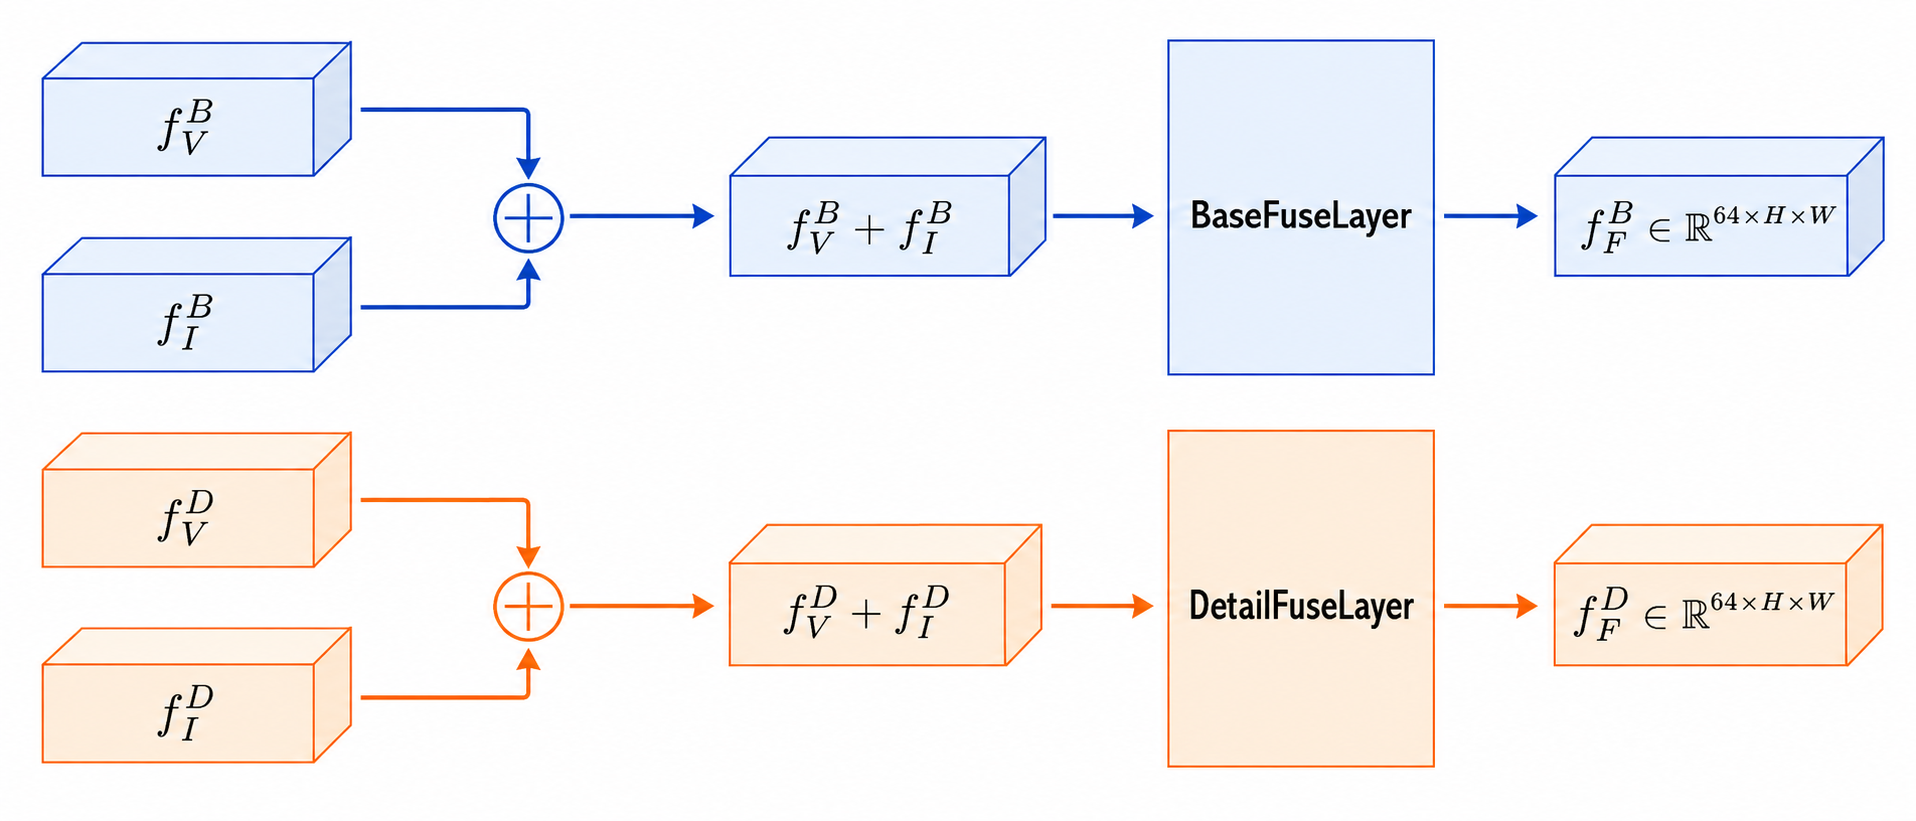
\includegraphics[width=\textwidth]{figures/fusion.png}
    \caption[Chi tiết Fusion Layer CDDFuse]{Chi tiết Fusion Layer: Base và Detail của hai modality được tổng hợp riêng biệt qua BaseFuseLayer và DetailFuseLayer. (Nguồn: \cite{zhao2023cddfuse})}
    \label{fig:cddfuse-fusion}
\end{figure}

\paragraph{3. Restormer Decoder.}
Decoder nối hai đặc trưng Base và Detail (concatenate 128 kênh), giảm về 64 kênh qua tích chập $1\!\times\!1$, sau đó qua 4 Restormer block và output head ($64 \to 32 \to 1$ kênh, kết thúc bằng sigmoid).

\begin{figure}[H]
    \centering
    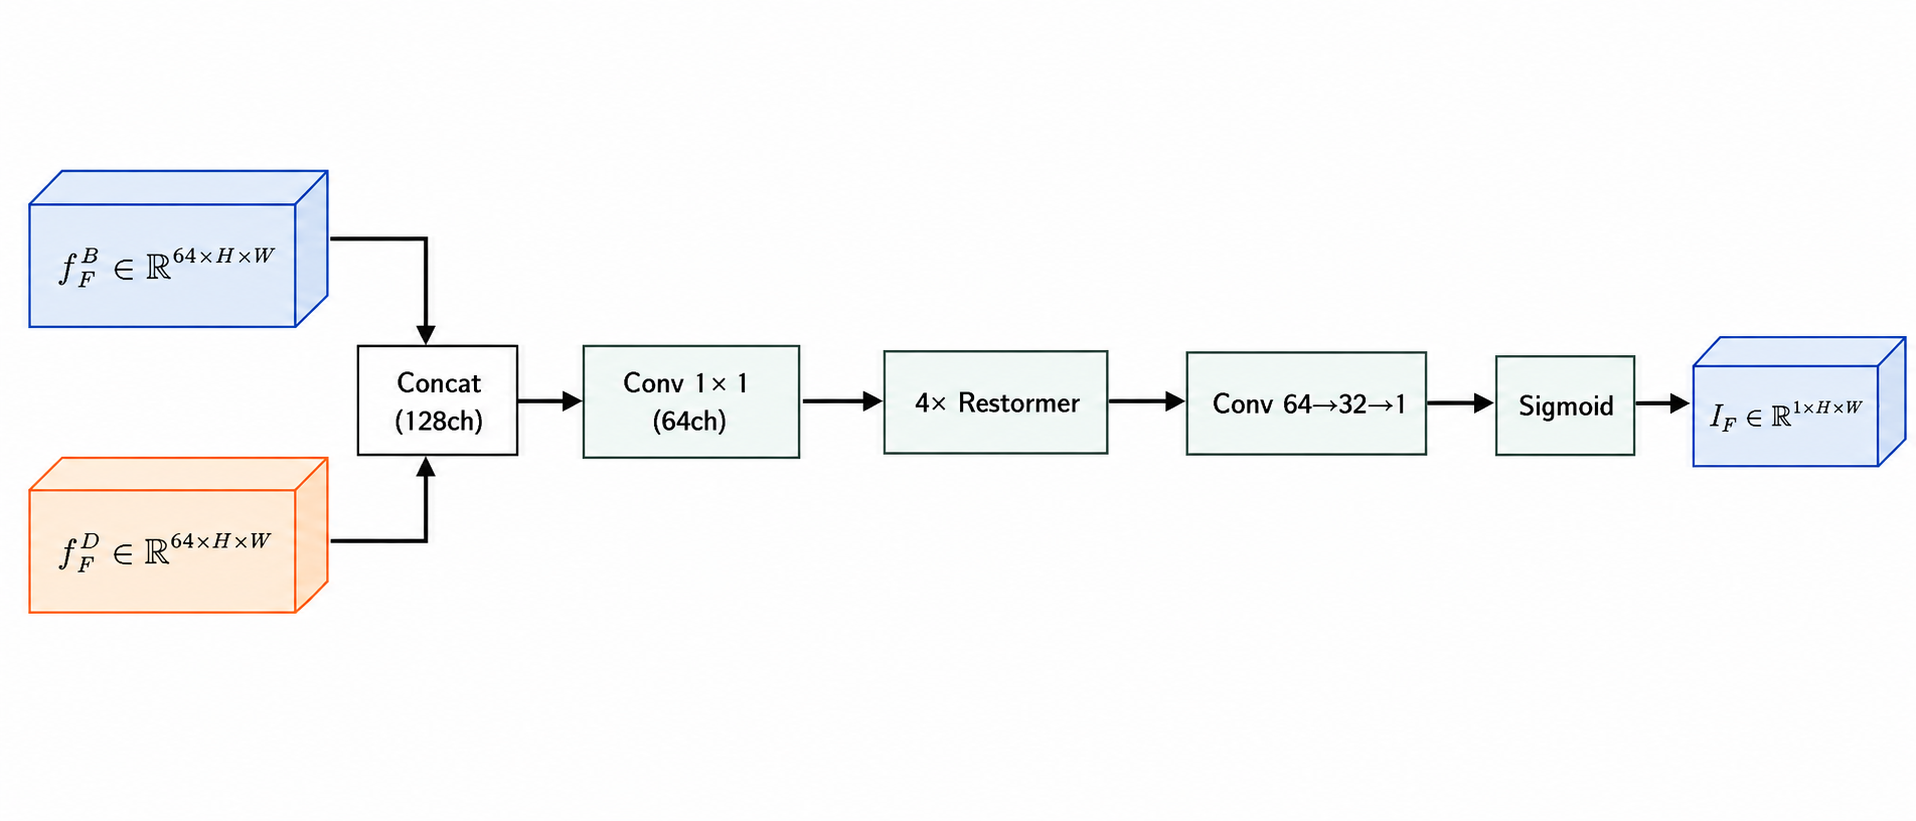
\includegraphics[width=\textwidth]{figures/decoder.png}
    \caption[Chi tiết kiến trúc Decoder CDDFuse]{Chi tiết kiến trúc Decoder CDDFuse: concat đặc trưng Base và Detail đã fusion, tái tạo ảnh đầu ra $I_F$ qua Restormer blocks và output head. (Nguồn: \cite{zhao2023cddfuse})}
    \label{fig:cddfuse-decoder}
\end{figure}

\paragraph{Tổng tham số.}
CDDFuse có $\sim 1{,}20$M tham số tổng cộng, phân bổ: Encoder ($\sim 50\%$), Decoder ($\sim 42\%$), Fusion Layer ($\sim 7\%$) và $\sim 8{,}200$ tham số tại phép cộng/các layer trong Fusion. Đây là mô hình nhẹ so với nhiều phương pháp SOTA (DDFM 200M+, U2Fusion 6.4M).

% ----------------------------------------------------------------
\subsection{Hàm mất mát và quy trình huấn luyện hai pha}
\label{ssec:cddfuse-loss}

CDDFuse áp dụng curriculum learning với hai pha huấn luyện tách biệt:

\paragraph{Pha I (epoch 0--39, tiền huấn luyện phân rã).}
Chỉ Encoder và Decoder được huấn luyện. Mỗi modality tự encode-decode (không có cross-modality fusion):
\begin{equation}
L_I = \alpha_1 (L_{\mathrm{recon}}^{V} + L_{\mathrm{recon}}^{I}) + \alpha_2 L_{\mathrm{decomp}} + \alpha_3 L_{\mathrm{TV}}
\end{equation}
Trong đó:
\begin{itemize}\itemsep1pt
    \item $L_{\mathrm{recon}}^{X} = 5 \cdot L_{\mathrm{SSIM}}(X, \hat{X}) + L_{\mathrm{MSE}}(X, \hat{X})$: buộc Decoder tái tạo lại ảnh gốc.
    \item $L_{\mathrm{decomp}} = \dfrac{(\mathrm{CC}_D)^2}{1.01 + \mathrm{CC}_B}$: Correlation-Driven loss cốt lõi. Tử số ép correlation của Detail hai modality về 0 (Detail cần mang thông tin riêng biệt); mẫu số thưởng khi Base hai modality tương quan cao (Base cần mang thông tin chung).
    \item $L_{\mathrm{TV}} = \|\nabla I_V - \nabla \hat{I}_V\|_1$: bảo toàn gradient biên.
\end{itemize}
Hệ số: $\alpha_1 = 1$, $\alpha_2 = 2$, $\alpha_3 = 5$ (theo code release).

\paragraph{Pha II (epoch 40--119, huấn luyện fusion).}
BaseFuseLayer và DetailFuseLayer được huấn luyện cùng với Encoder/Decoder:
\begin{align}
L_{II} &= L_{\mathrm{fusion}} + \alpha_4 L_{\mathrm{decomp}} \\
L_{\mathrm{int}}^{II} &= \|\hat{I}_F - \max(I_V, I_I)\|_F^2 \label{eq:lint} \\
L_{\mathrm{grad}}^{II} &= \|\nabla \hat{I}_F - \max(|\nabla I_V|, |\nabla I_I|)\|_1
\end{align}
Hàm mất mát này yêu cầu ảnh tổng hợp giữ nguyên pixel sáng hơn từ hai nguồn và gradient lớn hơn tại mỗi điểm, đảm bảo không mất thông tin từ modality nào.

\paragraph{Cấu hình huấn luyện.} Optimizer: Adam riêng cho mỗi thành phần. Learning rate: $10^{-4}$, StepLR $\gamma = 0.5$ mỗi 20 epoch. Batch size: 8. Patch $128\!\times\!128$. Gradient clipping: norm max $0.01$.

% ----------------------------------------------------------------
\subsection{Vị trí CDDFuse trong bức tranh SOTA}
\label{ssec:cddfuse-sota}

Để xác định vị trí của CDDFuse và lý do chọn làm base model, đồ án đánh giá 22 phương pháp trên cùng tập test Harvard 72 cặp ảnh với 22 chỉ số chất lượng, xếp hạng bằng Composite Z-score (chi tiết tại Mục~\ref{sec:zscore-per-modal}).

\begin{table}[H]
\centering
\small
\caption{Xếp hạng 22 phương pháp tổng hợp ảnh y tế theo Composite Z-score. Đánh giá trên 72 cặp ảnh test, 22 chỉ số chất lượng, gộp ba modality CT/PET/SPECT.}
\label{tab:zscore-ranking}
\begin{tabular}{rlc|rlc}
\toprule
\textbf{Rank} & \textbf{Model} & \textbf{$\bar{z}$} & \textbf{Rank} & \textbf{Model} & \textbf{$\bar{z}$} \\
\midrule
1  & MM-Net-Fusion          & $+1.029$ & 12 & DDBFusion         & $+0.040$ \\
\textbf{2}  & \textbf{CDDFuse} \cite{zhao2023cddfuse} & $\mathbf{+0.926}$ & 13 & AdaFuse           & $+0.027$ \\
3  & MFS-Fusion             & $+0.688$ & 14 & AWFusion          & $-0.145$ \\
4  & CM-CSAMFNet            & $+0.591$ & 15 & PSFusion          & $-0.148$ \\
5  & BSAFusion              & $+0.576$ & 16 & MLFuse            & $-0.358$ \\
6  & MMIF-INet              & $+0.440$ & 17 & WaveFusion        & $-0.374$ \\
7  & LRFNet                 & $+0.410$ & 18 & NestFuse          & $-0.535$ \\
8  & CMMDL                  & $+0.185$ & 19 & TUFusion          & $-0.673$ \\
9  & GeSeNet                & $+0.144$ & 20 & ITFuse            & $-0.861$ \\
10 & MBHFuse                & $+0.076$ & 21 & MMAE              & $-0.994$ \\
11 & ECINFusion             & $+0.063$ & 22 & C2RF              & $-1.105$ \\
\bottomrule
\end{tabular}
\end{table}

CDDFuse đứng vị trí thứ 2 với $\bar{z} = 0{,}926$. Lý do chọn CDDFuse thay vì MM-Net-Fusion (rank 1): khoảng cách composite z chỉ $0{,}10$, trong khi CDDFuse có kiến trúc mô-đun hóa rõ ràng, tham số nhẹ ($1{,}2$M), mã nguồn và checkpoint được công bố đầy đủ, và có điểm cải tiến cụ thể tại Fusion Layer, đây là điều kiện lý tưởng để nghiên cứu tác động của fusion rule trong khuôn khổ đồ án.

% ================================================================
% ================================================================
\section{Phương pháp đánh giá chất lượng ảnh tổng hợp}
\label{sec:eval-bg}

\subsection{Các chỉ số chất lượng VIFB}
\label{ssec:metrics}

Đồ án sử dụng 22 chỉ số chất lượng theo chuẩn VIFB~\cite{liu2020vifb}, chia thành sáu nhóm theo bản chất đo lường. Phần này trình bày định nghĩa toán học chi tiết cho các chỉ số được sử dụng trực tiếp trong đánh giá và so sánh. Ký hiệu chung: $A$, $B$ là hai ảnh đầu vào (ví dụ MRI và CT), $F$ là ảnh tổng hợp đầu ra, kích thước $M \times N$.

% ── Nhóm 1: Thông tin ─────────────────────────────────────────────────────────
\subsubsection*{Nhóm 1: Thông tin}

\paragraph{Entropy (EN).}
Đo lượng thông tin trung bình trong ảnh tổng hợp, tính theo histogram xác suất cường độ điểm ảnh:
\begin{equation}
\mathrm{EN}(F) = -\sum_{l=0}^{L-1} p_l \log_2 p_l
\end{equation}
trong đó $p_l$ là xác suất xuất hiện mức cường độ $l$ (histogram chuẩn hóa), $L=256$. Giá trị cao hơn cho thấy ảnh fused phong phú thông tin hơn. $\uparrow$ cao tốt hơn.

\paragraph{Mutual Information (MI).}
Đo lượng thông tin chung được bảo toàn từ cả hai nguồn vào ảnh fused:
\begin{equation}
\mathrm{MI}(A,B;F) = \mathrm{MI}(A;F) + \mathrm{MI}(B;F)
\end{equation}
trong đó $\mathrm{MI}(X;F) = \sum_{x,f} p_{XF}(x,f)\log\frac{p_{XF}(x,f)}{p_X(x)\,p_F(f)}$ với $p_{XF}$ là phân phối xác suất đồng thời. $\uparrow$ cao tốt hơn.

\paragraph{Cross Entropy (CE).}
Đo sự khác biệt phân phối xác suất giữa ảnh đầu vào và ảnh fused:
\begin{equation}
\mathrm{CE}(A,F) = \sum_l p_A(l)\log\frac{p_A(l)}{p_F(l)}
\end{equation}
Tổng CE từ cả hai nguồn: $\mathrm{CE} = \mathrm{CE}(A,F)+\mathrm{CE}(B,F)$. Giá trị thấp hơn nghĩa là ảnh fused phân phối cường độ gần với nguồn hơn. $\downarrow$ thấp tốt hơn.

\paragraph{QMI (Normalized Mutual Information).}
Phiên bản chuẩn hóa của MI, ổn định hơn khi so sánh giữa các modality:
\begin{equation}
\mathrm{QMI}(A,B;F) = \frac{\mathrm{MI}(A;F)}{H(A)+H(F)} + \frac{\mathrm{MI}(B;F)}{H(B)+H(F)}
\end{equation}
trong đó $H(\cdot)$ là entropy. $\uparrow$ cao tốt hơn.

% ── Nhóm 2: Cấu trúc ─────────────────────────────────────────────────────────
\subsubsection*{Nhóm 2: Cấu trúc}

\paragraph{SSIM (Structural Similarity Index).}
Đo độ tương đồng cấu trúc giữa ảnh fused và ảnh tham chiếu dựa trên luminance, contrast và structure~\cite{wang2004ssim}:
\begin{equation}
\mathrm{SSIM}(X,F) = \frac{(2\mu_X\mu_F+c_1)(2\sigma_{XF}+c_2)}{(\mu_X^2+\mu_F^2+c_1)(\sigma_X^2+\sigma_F^2+c_2)}
\end{equation}
trong đó $\mu$, $\sigma^2$, $\sigma_{XF}$ lần lượt là mean, variance và cross-covariance; $c_1,c_2$ là hằng số ổn định. Trong bài toán MIF không có ground truth, SSIM được tính so với cả hai nguồn và cộng: $\mathrm{SSIM}=\mathrm{SSIM}(A,F)+\mathrm{SSIM}(B,F)$. $\uparrow$ cao tốt hơn.

\paragraph{SD (Standard Deviation).}
Đo độ tương phản tổng thể của ảnh fused:
\begin{equation}
\mathrm{SD}(F) = \sqrt{\frac{1}{MN}\sum_{i=1}^{M}\sum_{j=1}^{N}\bigl(F_{ij}-\bar{F}\bigr)^2}
\end{equation}
Giá trị cao hơn phản ánh vùng sáng--tối phân biệt rõ hơn, nội dung hình ảnh phong phú hơn. $\uparrow$ cao tốt hơn.

% ── Nhóm 3: Biên và gradient ─────────────────────────────────────────────────
\subsubsection*{Nhóm 3: Biên và gradient}

\paragraph{Spatial Frequency (SF).}
Đo mức độ hoạt động tần số không gian tổng thể của ảnh fused~\cite{eskicioglu1995sf}:
\begin{equation}
\mathrm{SF}(F) = \sqrt{RF^2 + CF^2}
\end{equation}
trong đó $RF = \sqrt{\frac{1}{MN}\sum_{i,j}(F_{i,j}-F_{i,j-1})^2}$ (Row Frequency) và $CF = \sqrt{\frac{1}{MN}\sum_{i,j}(F_{i,j}-F_{i-1,j})^2}$ (Column Frequency). Giá trị cao hơn nghĩa là ảnh fused có nhiều chi tiết kết cấu và biên hơn. $\uparrow$ cao tốt hơn.

\paragraph{Average Gradient (AG).}
Đo độ sắc nét trung bình của ảnh fused thông qua gradient cục bộ~\cite{cui2015ag}:
\begin{equation}
\mathrm{AG}(F) = \frac{1}{MN}\sum_{i=1}^{M}\sum_{j=1}^{N} \sqrt{\frac{(\partial F/\partial x)^2 + (\partial F/\partial y)^2}{2}}
\end{equation}
trong đó $\partial F/\partial x$, $\partial F/\partial y$ là đạo hàm riêng theo hướng ngang và dọc. Giá trị cao hơn phản ánh ảnh fused sắc nét, bảo toàn tốt chi tiết biên. $\uparrow$ cao tốt hơn.

\paragraph{Edge Intensity (EI).}
Đo cường độ biên tổng thể sử dụng bộ lọc Laplacian~\cite{liu2020vifb}:
\begin{equation}
\mathrm{EI}(F) = \frac{1}{MN}\sum_{i,j}\bigl|\nabla^2 F_{ij}\bigr|
\end{equation}
trong đó $\nabla^2$ là toán tử Laplacian. EI tương quan chặt với AG nhưng nhấn mạnh các biên đột ngột (high-frequency). $\uparrow$ cao tốt hơn.

\paragraph{$Q^{AB/F}$ (Qabf, Petrovic).}
Đánh giá mức độ truyền tải thông tin gradient--biên từ hai ảnh nguồn vào ảnh fused~\cite{xydeas2000objective}:
\begin{equation}
Q^{AB/F} = \frac{\sum_{i,j}\bigl(Q^{AF}_{ij}\,w^A_{ij} + Q^{BF}_{ij}\,w^B_{ij}\bigr)}{\sum_{i,j}(w^A_{ij}+w^B_{ij})}
\end{equation}
trong đó $Q^{XF}_{ij}$ là chỉ số truyền biên tại điểm $(i,j)$, $w^X_{ij}$ là trọng số tầm quan trọng cạnh. $Q^{AB/F}\in[0,1]$; giá trị 1 nghĩa là toàn bộ thông tin biên từ cả hai nguồn được giữ lại hoàn toàn. $\uparrow$ cao tốt hơn.

\paragraph{NABF (Noise/Artifact at Boundary Fusion).}
Đo lượng artifact biên xuất hiện trong ảnh fused nhưng không có trong cả hai nguồn:
\begin{equation}
\mathrm{NABF} = \frac{\sum_{i,j}\bigl(Q^{FA}_{ij}\,w^{FA}_{ij} + Q^{FB}_{ij}\,w^{FB}_{ij}\bigr)}{\sum_{i,j}(w^{FA}_{ij}+w^{FB}_{ij})}
\end{equation}
Giá trị NABF cao nghĩa là ảnh fused tạo thêm artifact biên không có trong nguồn gốc. $\downarrow$ thấp tốt hơn.

% ── Nhóm 4: Wavelet ───────────────────────────────────────────────────────────
\subsubsection*{Nhóm 4: Wavelet}

\paragraph{QM (Piella Wavelet Quality).}
Đánh giá chất lượng tổng hợp dựa trên tương quan cấu trúc tại nhiều mức phân giải trong miền wavelet~\cite{piella2003new}:
\begin{equation}
Q_M = \frac{1}{W}\sum_w \lambda_w(F)\bigl[Q_0(A,F|w)\,c(A,F|w) + Q_0(B,F|w)\,c(B,F|w)\bigr]
\end{equation}
trong đó $w$ là chỉ số mức wavelet, $\lambda_w$ là trọng số saliency, $Q_0$ là SSIM cục bộ trong miền wavelet, $c(\cdot)$ là hệ số tương quan. QM nhạy với việc bảo toàn chi tiết tần số cao (cạnh, texture). $\uparrow$ cao tốt hơn.

% ── Tóm tắt ───────────────────────────────────────────────────────────────────
\subsubsection*{Tóm tắt và phân nhóm sử dụng}

\begin{table}[H]
\centering
\small
\caption{12 chỉ số chính sử dụng trong đánh giá, phân loại theo nhóm và hướng tốt.}
\label{tab:metrics-summary}
\setlength{\tabcolsep}{5pt}
\begin{tabular}{llll}
\toprule
\textbf{Nhóm} & \textbf{Chỉ số} & \textbf{Hướng} & \textbf{Ý nghĩa} \\
\midrule
Thông tin   & EN            & $\uparrow$   & Lượng thông tin ảnh fused \\
            & MI            & $\uparrow$   & Thông tin chung từ nguồn vào fused \\
            & CE            & $\downarrow$ & Sai lệch phân phối xác suất \\
            & QMI           & $\uparrow$   & MI chuẩn hóa \\
\midrule
Cấu trúc    & SSIM          & $\uparrow$   & Độ tương đồng cấu trúc \\
            & SD            & $\uparrow$   & Độ tương phản tổng thể \\
            & PSNR          & $\uparrow$   & Tỷ lệ tín hiệu/nhiễu \\
\midrule
Biên/grad.  & SF            & $\uparrow$   & Tần số không gian \\
            & AG            & $\uparrow$   & Gradient trung bình \\
            & EI            & $\uparrow$   & Cường độ biên \\
            & Qabf          & $\uparrow$   & Truyền tải biên (Petrovic) \\
            & NABF          & $\downarrow$ & Artifact biên \\
\midrule
Wavelet     & QM            & $\uparrow$   & Chất lượng đa phân giải \\
\bottomrule
\end{tabular}
\end{table}

Các chỉ số trong cùng nhóm thường có tương quan cao với nhau. Một cải thiện thực sự cần thể hiện đồng thời trên cả nhóm chỉ số liên quan, không chỉ trên một metric đơn lẻ.

Tóm lại, Chương~\ref{ch:background} đã trình bày đầy đủ nền tảng lý thuyết từ biểu diễn dữ liệu ảnh, kiến trúc mạng nơ-ron, đến mô hình CDDFuse và phương pháp đánh giá. Trên cơ sở đó, Chương~\ref{ch:method} tiếp theo sẽ trình bày phương pháp CDDFuse-AG đề xuất.
